
\chapter{相关研究综述}
\label{chap:relatedwork}
流行度预测问题自被提出以来,受到了学术界和产业界的广泛关注。本章从流行度的统计特征分析、流行度预测方法以及流行度预测问题的可预测性三个方面入手,对流行度预测领域的相关工作进行了系统的总结和归纳,以便读者更好地了解和掌握该领域的相关知识,进而更好地理解本文的工作。

\section{流行度的统计特征分析}
在线内容的流行度分析工作最早源于网站缓存策略的研究。Cunha等人\citep{cunha1995characteristics}在研究站点中网页的访问情况时发现,网页被访问频率的分布服从Zipf定律\citep{zipf2016human},也就是说:流行度排名为$i$的网页被用户访问的概率正比于$1/i$,如图\ref{fig:pageDist}所示。这一现象表明,网页的访问频次分布是不均匀的。Almeida等人\citep{almeida1996characterizing}在研究万维网中所有网页的访问频次时,也发现了同样的分布规律。
\begin{figure}[!htbp]
  \centering
  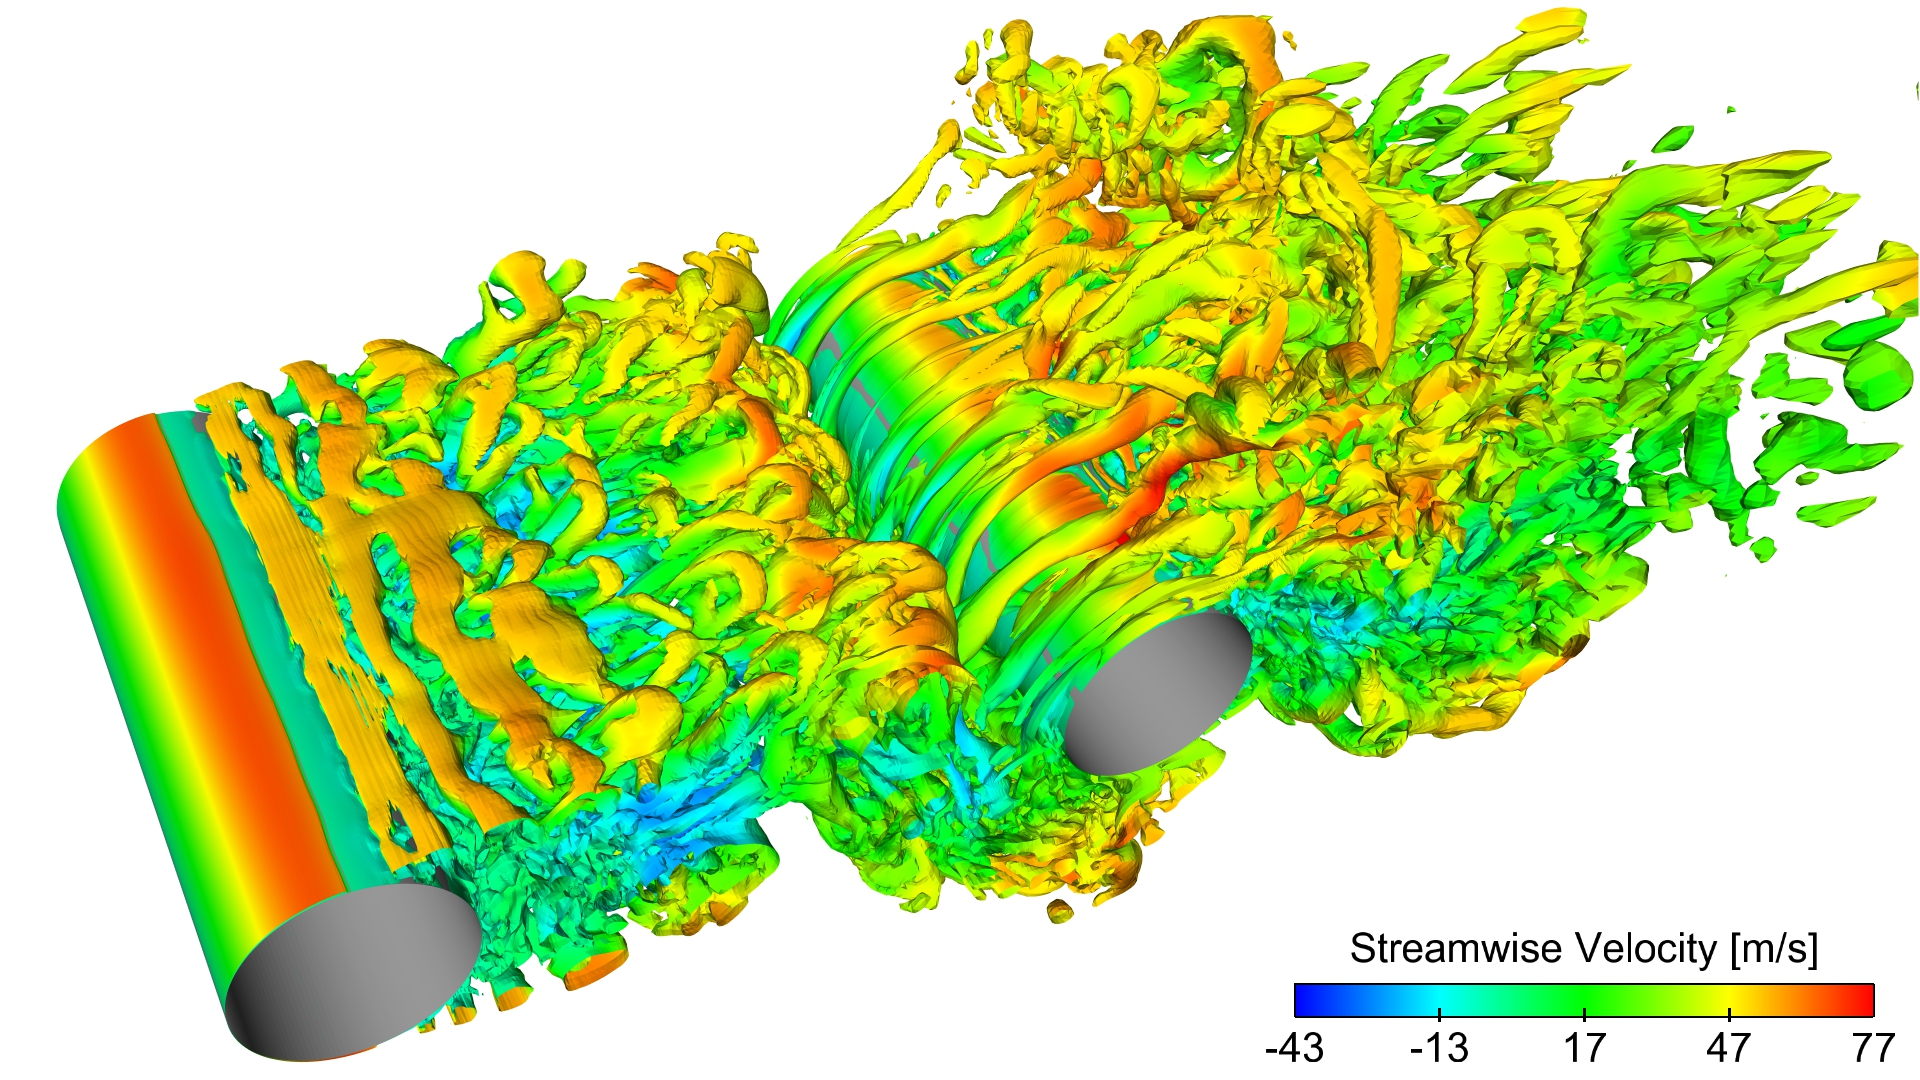
\includegraphics[width=0.45\textwidth]{ITC_Q_Criteria}
  \caption{Q判据等值面图}
  \label{fig:pageDist}
\end{figure}

随着信息技术的发展,视频分享类网站和社交网络平台不断涌现,也引起了研究人员的关注。Gill等人\citep{gill2007youtube}收集并分析了视频网站Youtube\footnote{\url{https://www.youtube.com}}上视频的访问数据,发现视频的访问频次信息依然服从Zipf定律。Cha等人\citep{cha2009analyzing}对Youtube网站上的视频数据进行了详细的分析,发现网站中不同类别下的视频的观看数分布都服从幂律分布。Kwak等人\citep{kwak2010twitter}研究了社交网络平台Twitter\footnote{\url{https://twitter.com}}上消息的转发情况,发现参与消息转发的人数服从幂律分布,如图\ref{fig:tweetDist}所示。
\begin{figure}[!htbp]
  \centering
  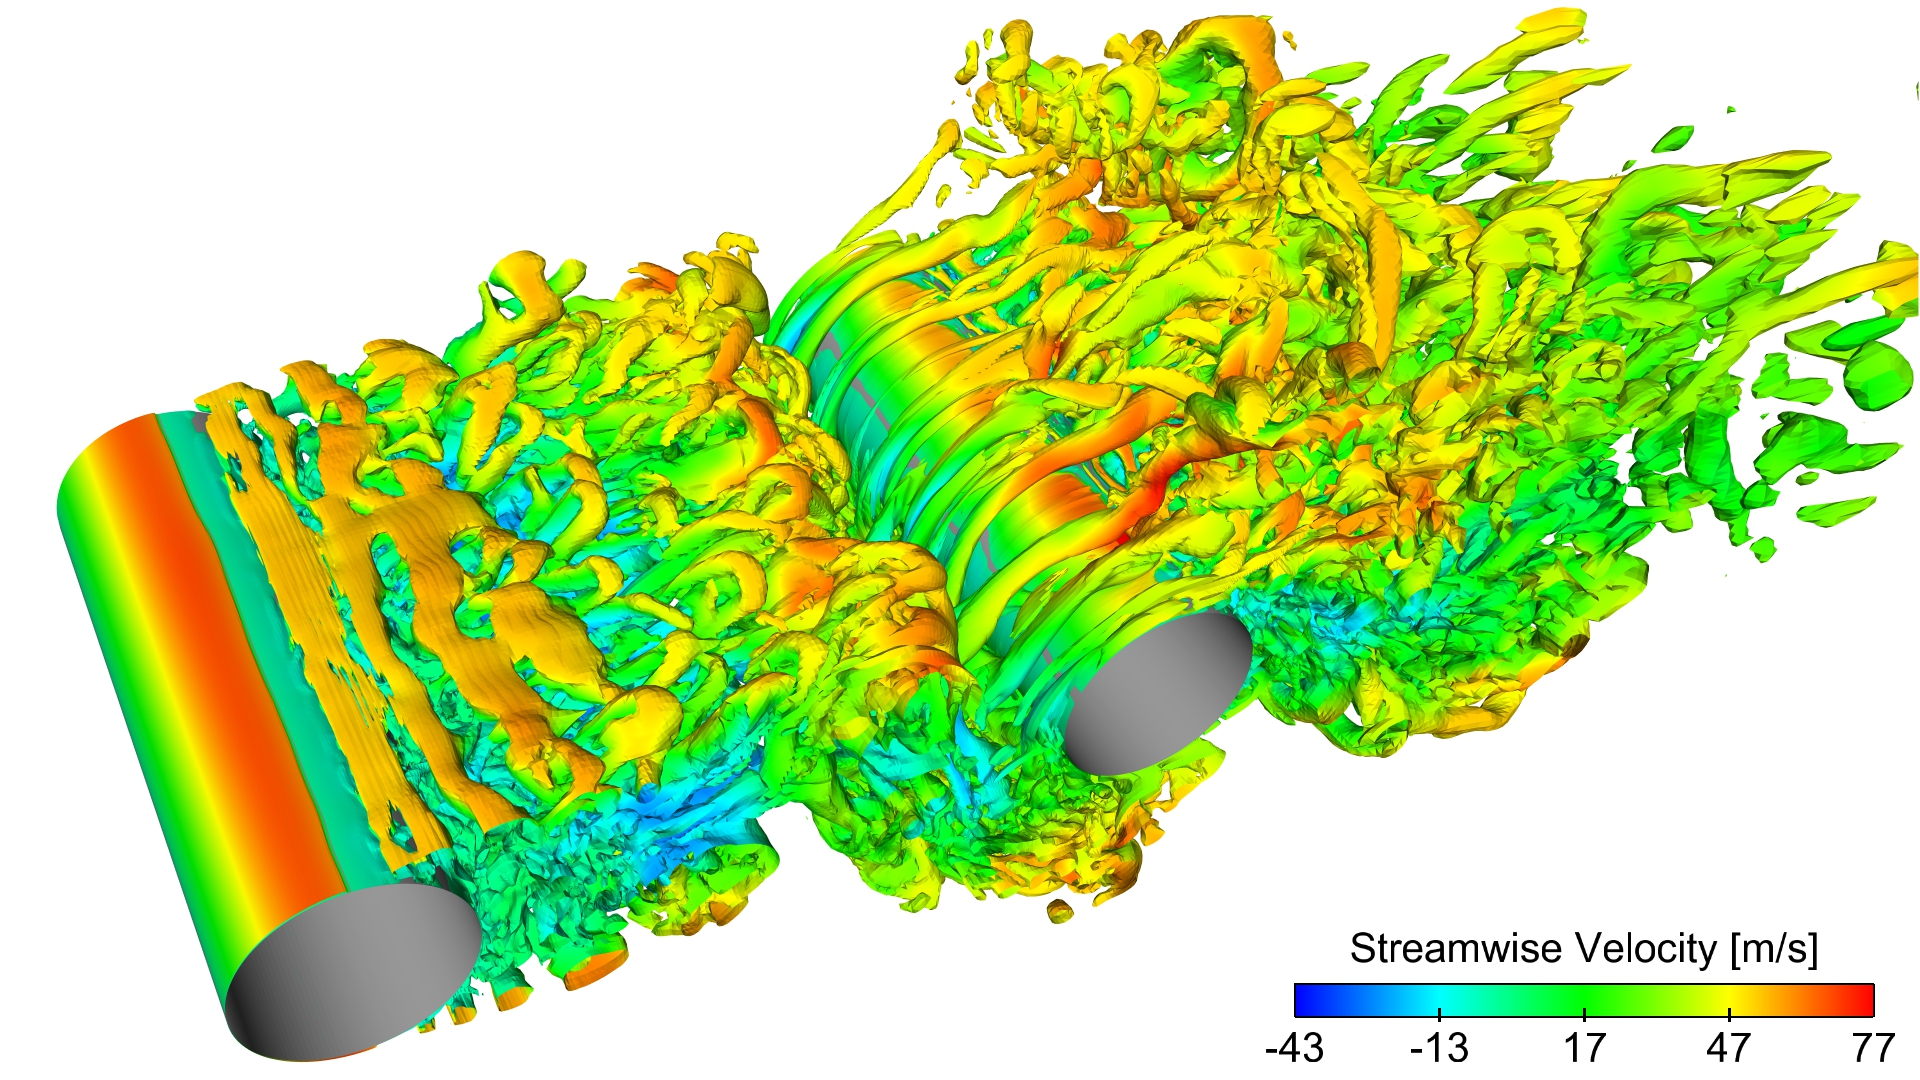
\includegraphics[width=0.45\textwidth]{ITC_Q_Criteria}
  \caption{Q判据等值面图}
  \label{fig:tweetDist}
\end{figure}

除了对宏观的流行度统计量的分析之外,还有一部分工作研究了流行度增长过程中的微观统计特征。Barabasi等人\citep{barabasi05}研究了人类的行为数据,发现人类的行为模式并不是服从传统方法中假设的泊松过程,而是存在爆发现象,并提出了一种基于事件优先级的排队模型来解释这一现象。爆发现象是指人类在参与某类事件时,大部分时间都处于沉寂状态,不会采取任何行为动作;中间夹杂了少数爆发区域,在爆发区域内会有大量的行为数据产生,如图\ref{fig:burst}所示。

爆发现象在在线内容的流行度增长过程中十分常见。Kaltenbrunner等人\citep{kaltenbrunner2007description}研究了新闻评论网站Slashdot\footnote{\url{https://slashdot.org}}上新闻的评论情况,并对评论数据的时间间隔分布进行了分析。统计结果表明,评论数据的时间间隔分布是两个log-normal分布的混合,并且存在明显的周期现象。Bao等人\citep{bao2013cumulative}研究了新浪微博中消息的转发时间间隔数据,发现转发时间间隔分布服从幂律分布,这也说明了社交网络中消息的流行度累积过程中存在爆发现象。
\begin{figure}[!htbp]
  \centering
  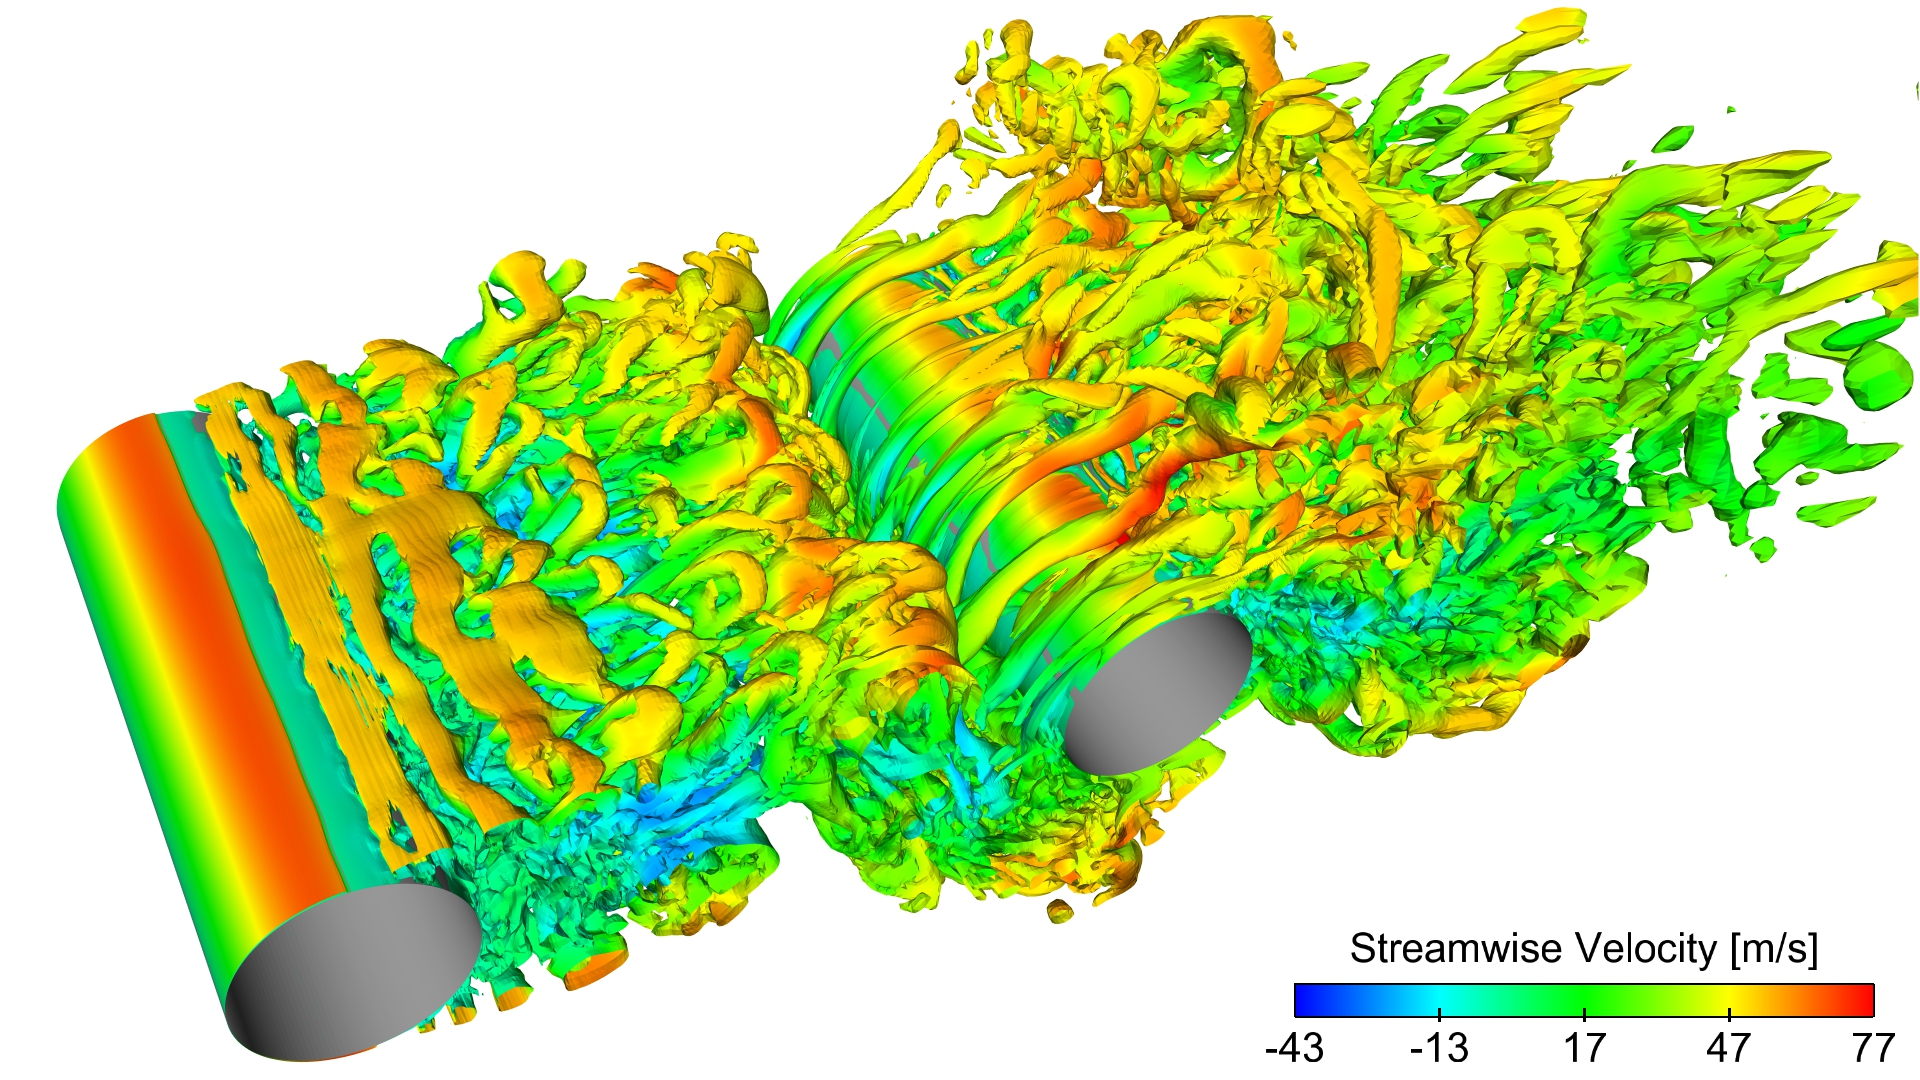
\includegraphics[width=0.45\textwidth]{ITC_Q_Criteria}
  \caption{Q判据等值面图}
  \label{fig:burst}
\end{figure}

除爆发现象外,研究人员还发现流行度的增长过程中存在着固定的模式。Yang等人\citep{yang2011patterns}研究了Twitter平台上消息的传播过程,提出了K-SC(K-Spectral Centroid)聚类方法,对消息的流行度变化过程进行聚类,将消息的流行度变化过程聚为六类,如图\ref{fig:pattern}所示。Crane等人\citep{crane2008robust}在研究Yotube网站中视频的观看数据时发现,视频的观看到达时间服从幂律分布,呈现出明显的``爆发-衰落"现象。此外,Costa等人\citep{ferraz2015rsc}还发现流行度的增长过程中呈现出明显的周期性特点。
\begin{figure}[!htbp]
  \centering
  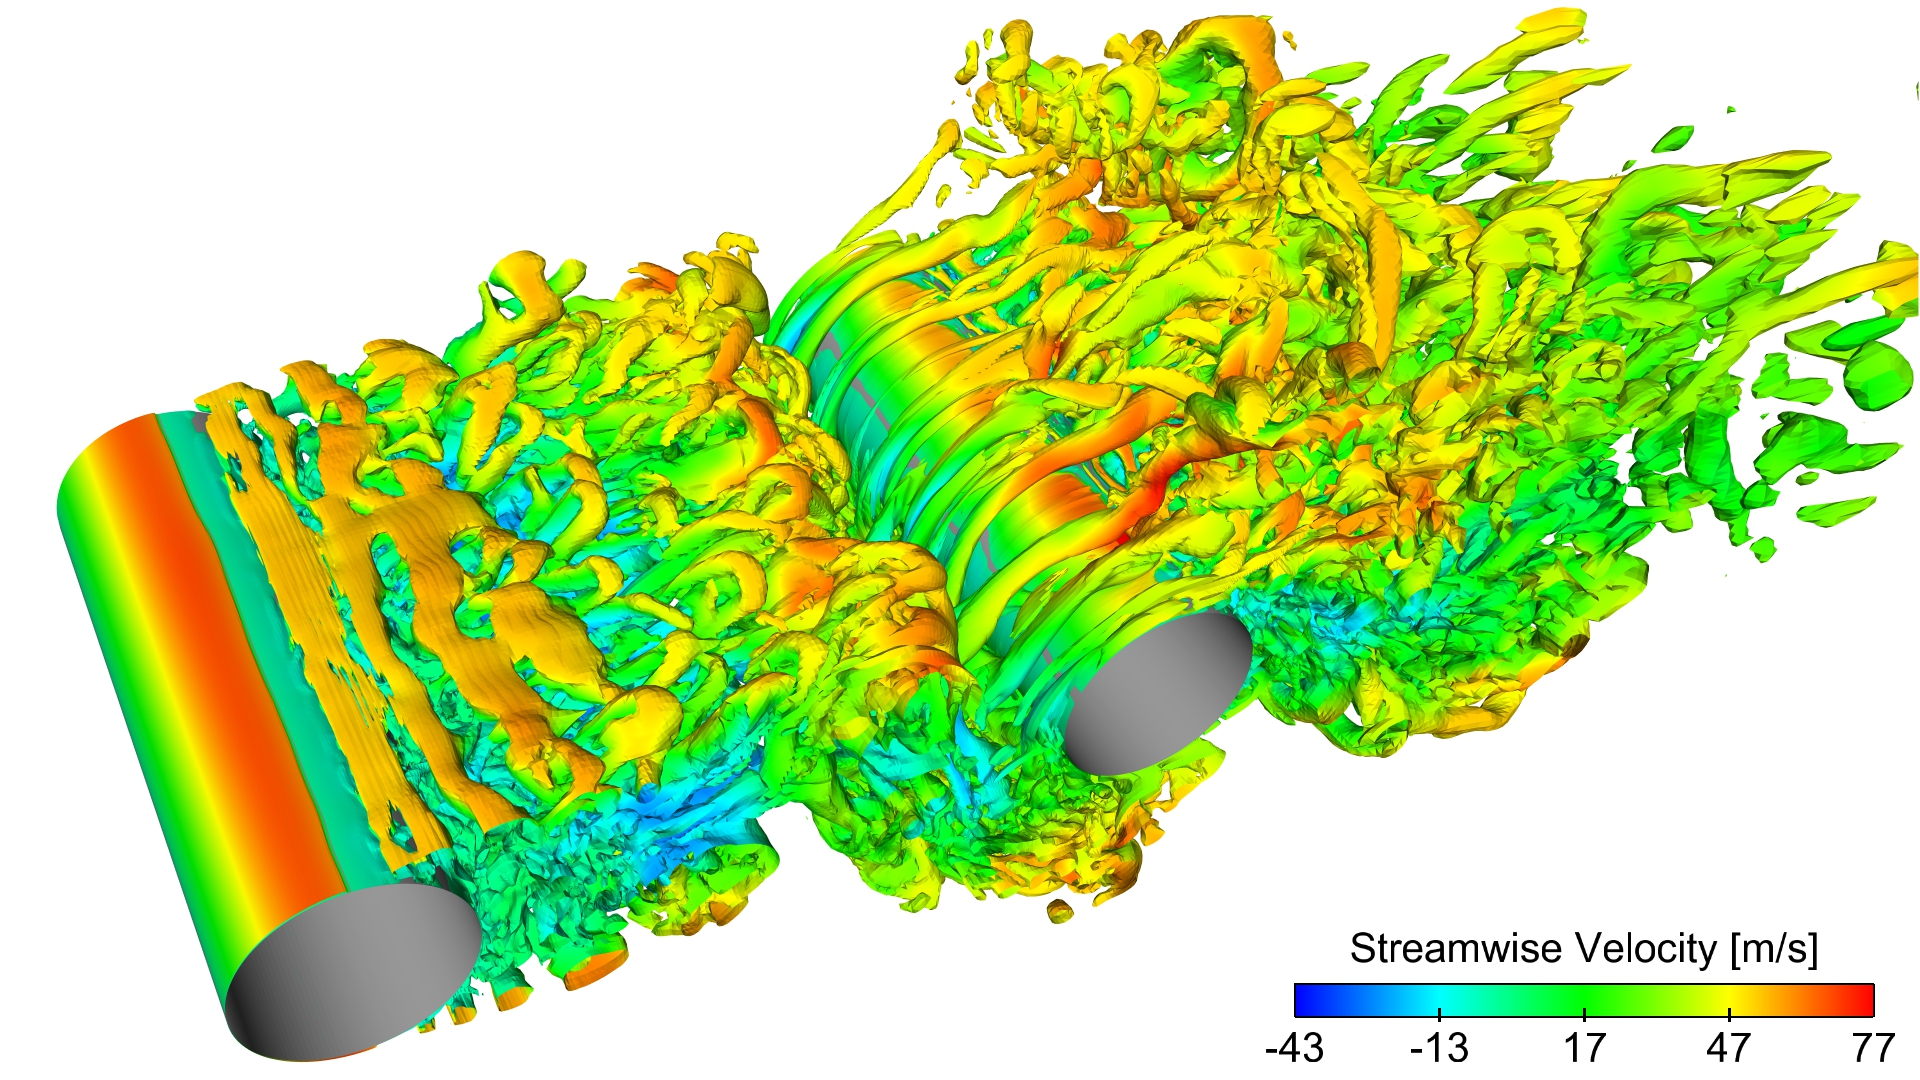
\includegraphics[width=0.45\textwidth]{ITC_Q_Criteria}
  \caption{Q判据等值面图}
  \label{fig:pattern}
\end{figure}

流行度分布的不均匀性,以及增长过程出现的爆发现象和时序特性,吸引了大量研究人员的关注,进而涌现出了多种流行度预测的模型和方法。
\section{流行度预测方法概述}
现有的流行度预测方法主要包含三类:基于特征的有监督学习方法、基于点过程的流行度到达过程建模方法和基于表示学习的方法。本节会依次对这三类方法进行介绍和总结。
\subsection{基于特征的有监督学习方法}
基于特征的流行度预测方法主要通过借助已有的有监督学习模型,结合人工抽取的特征,来对流行度的增长过程进行预测。在这类方法中,流行度预测问题通常会被形式化为分类或者回归问题:给定一组历史消息的各种特征信息以及消息在观测窗口$[0,T_r]$和预测窗口$[0,T_s]$内的流行度数据作为训练样本,利用现有的分类或回归方法学习得到预测模型,进而对待预测的消息的流行度作出预测。这类方法的核心在于寻找对于流行度预测有着重要指示作用的特征。常见的用于流行度预测的特征包括消息内容特征、用户特征、时序特征和传播级联的结构特征。
\begin{figure}[!htbp]
  \centering
  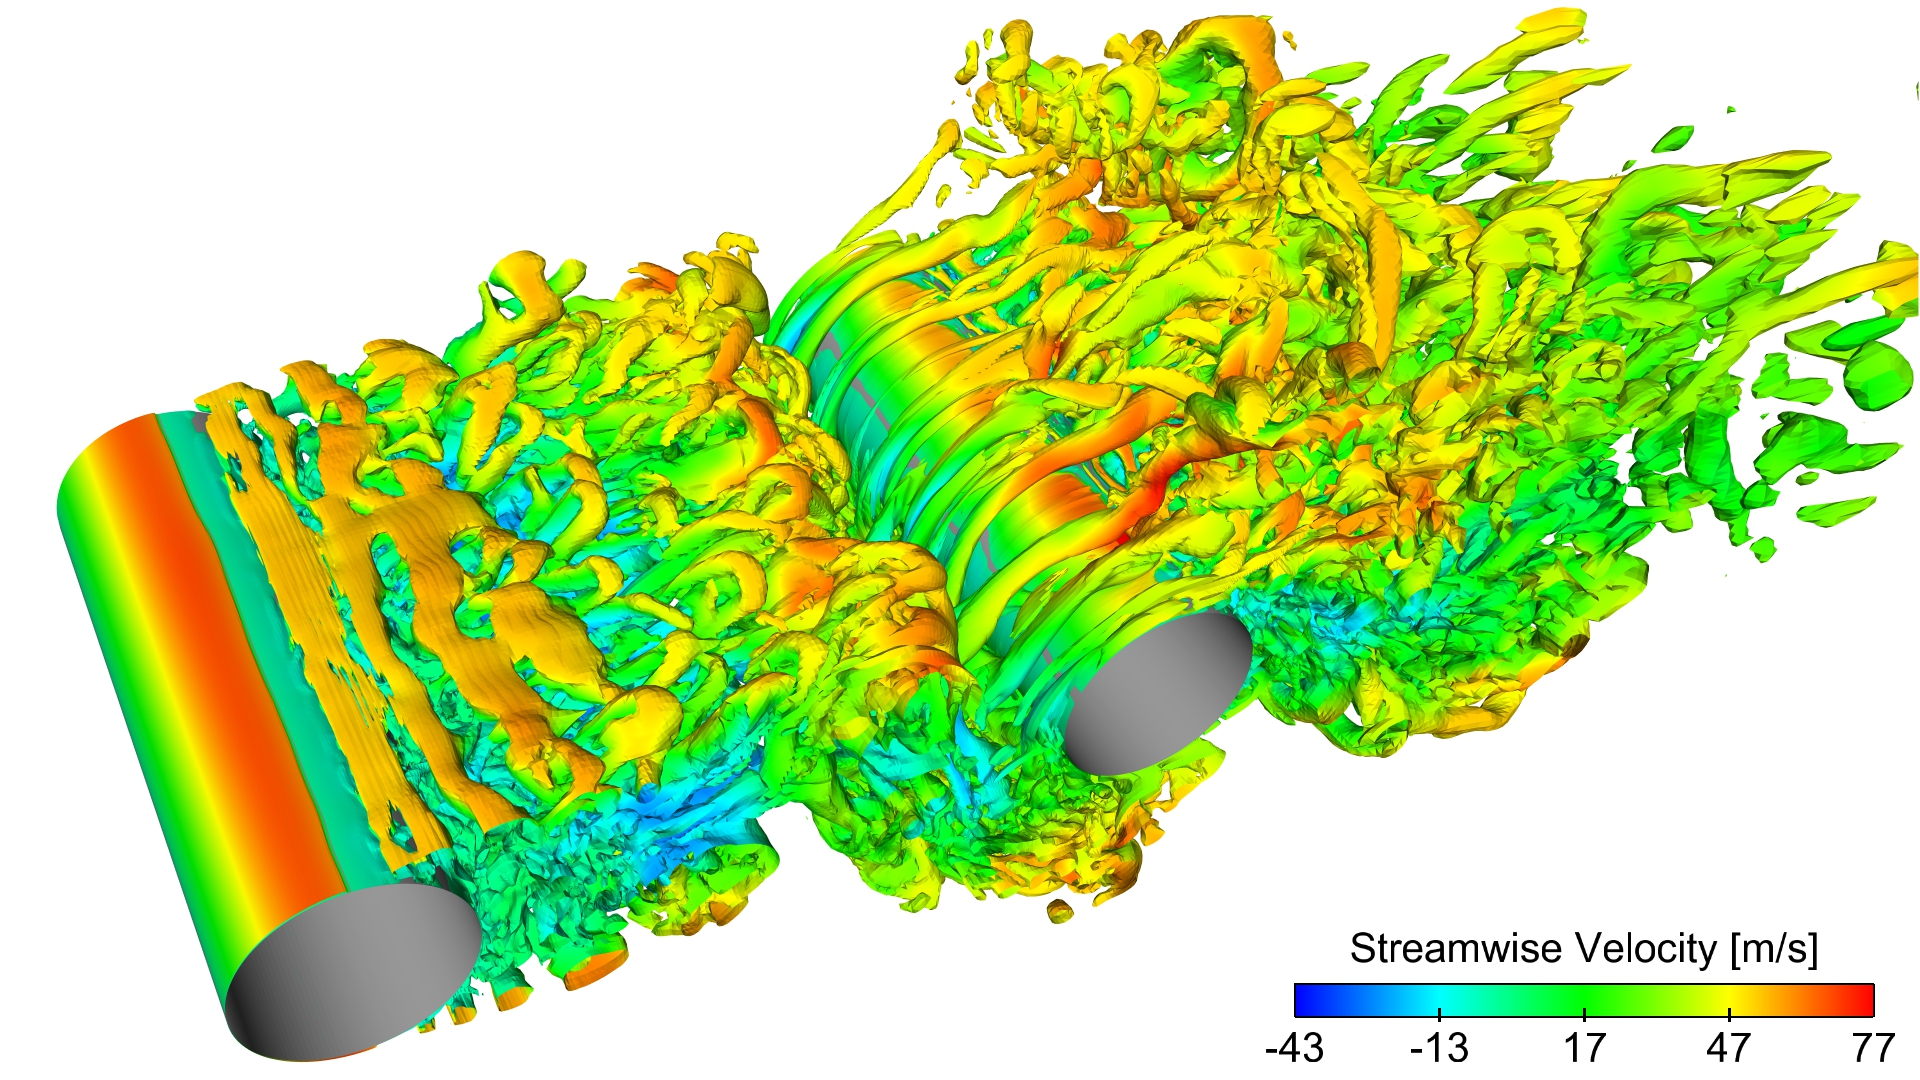
\includegraphics[width=0.45\textwidth]{ITC_Q_Criteria}
  \caption{Q判据等值面图}
  \label{fig:loglinear}
\end{figure}

时序特征方面,常用于流行度预测的时序特征包括观测窗口内的累积流行度特征和流行度时间序列特征。Cha等人\citep{cha2009analyzing}分析了Youtube网站上视频的流行度增长数据,发现视频上传7天后的访问量和视频上传后一天以及上传后两天的访问量之间存在着非常强的相关性,进而提出了预测视频近期流行度的任务,并指出视频上传后短期内的累计流行度是重要的指示特征。Szabo等人\citep{szabo2010predicting}研究了Digg\footnote{\url{http://digg.com}}网站上的新闻数据和Youtube网站上的视频数据,发现这些内容早期的流行度和后期的流行度在进行对数变换后,存在着非常强的线性相关性,如图\ref{fig:loglinear}所示。基于这一观测,作者提出了S-H(Szabo-Huberman)模型,将消息在观测窗口内的累积流行度作为特征,利用对数线性回归模型来预测消息在预测时刻的流行度。Gursun等人\citep{gursun2011describing}分析了Youtube网站中部分视频在上传后一年内完整的观看频次序列,发现可以根据将视频按照访问频次分为两类:长期流行的视频和短期流行的视频,并利用时间序列分析模型中的自回归移动平均模型(Autoregressive Moving Average,ARMA)\citep{marple1987digital},对长期流行的视频的流行度变化过程进行了预测。Pinto等人\citep{pinto2013using}研究了Youtube网站中视频的流行度时间序列数据。作者将视频在观测窗口等分为若干长度相等的区间,并抽取了各时间区间内视频的观看数的增长量作为特征。作者在研究视频的时间序列后发现S-H模型的假设存在着局限性:早期累计流行度相近的视频,后期的流行度变化过程可能会有很大的差距,如图\ref{fig:pinto}所示。作者提出将消息在观测窗口内的时间序列数据作为特征,利用多元线性回归模型来预测消息的流行度。
\begin{figure}[!htbp]
  \centering
  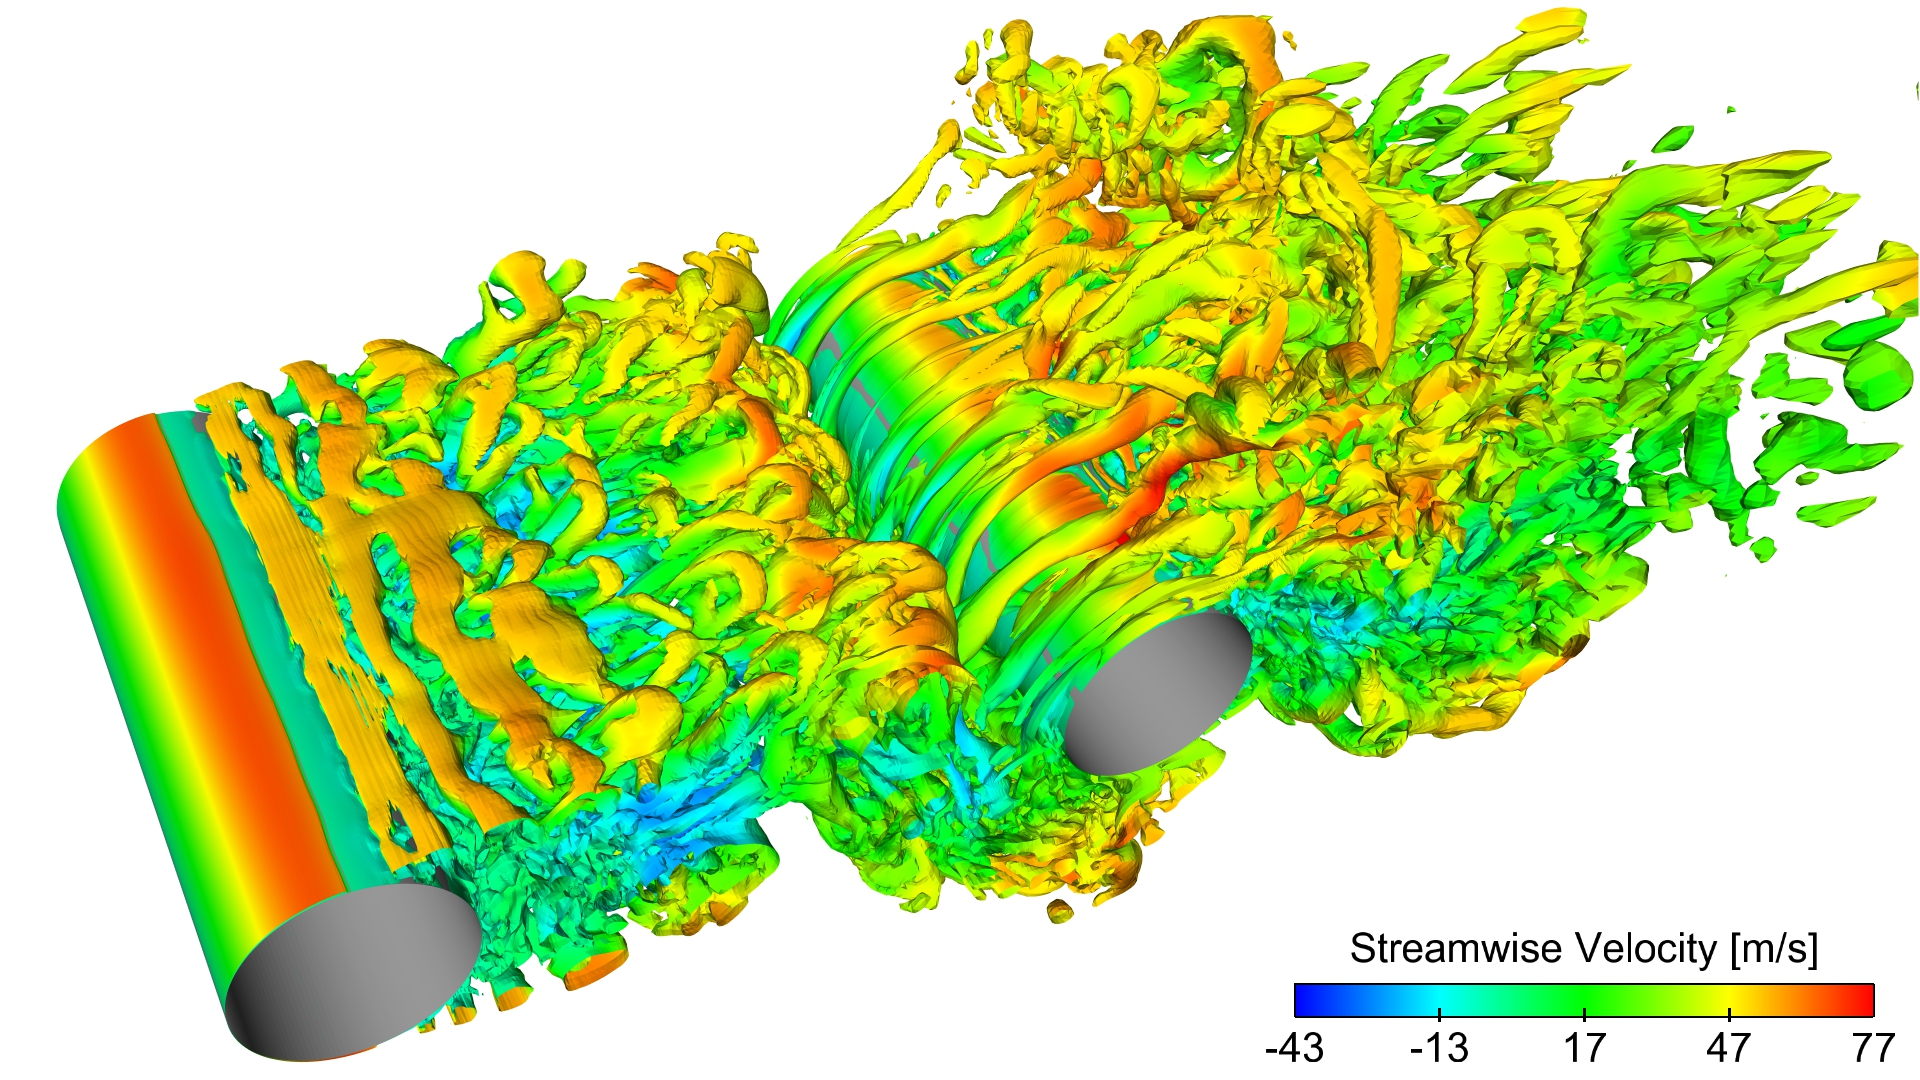
\includegraphics[width=0.45\textwidth]{ITC_Q_Criteria}
  \caption{Q判据等值面图}
  \label{fig:pinto}
\end{figure}

内容特征方面,Tsagkias等人\citep{tsagkias2009predicting}抽取了新闻的内容特征,来对新闻的评论数进行事前预测:在新闻发布之前,利用新闻的元信息,来预测新闻的评论数。作者将这一预测问题形式化为两阶段分类问题:新闻发布能否接收到评论,以及接收到的评论数会高还是低。在特征方面,作者抽取了新闻中重要性较高的前100个词的词频信息作为新闻的文本特征,新闻中包含的不同类型的命名实体的个数作为新闻的语义特征。此外,作者还抽取了新闻的其他元信息特征。实验结果表明,文本特征和语义特征对分类结果有较好的指示作用。Hong等人\citep{hong2011predicting}同样将Twitter平台中消息的流行度预测问题形式化为一个两阶段分类问题:消息是否会被转发以及消息最终的流行度等级。作者利用TF-IDF模型和LDA主题模型\citep{blei2003latent}来抽取消息的内容特征,同时结合网络拓扑结构特征以及时序特征来进行预测。Bandari等人\citep{bandari2012pulse}研究了新闻订阅站点Feedzilla\footnote{\url{http://news.feedzilla.com}}的数据在Twitter平台上的流行度情况。作者抽取了新闻的四类内容特征来进行预测,包括新闻所属的类别、新闻源站点的信息、新闻的倾向性特征和新闻中包含的命名实体。作者分别使用回归和分类模型对新闻的流行度进行了预测,得到了很好的预测效果。Bian等人\citep{bian2014predicting}研究了腾讯微博\footnote{\url{http://t.qq.com}}中消息的传播情况和用户的参与情况,从兴趣导向、社交影响和病毒式传播三个方面,建模了用户和消息之间的相互作用,进而对消息的流行度和用户的参与情况进行预测。建模过程中,作者提出了一种多任务迁移模型来建模消息的内容,提取出消息中的主题信息,用于后续的预测任务。

用户特征方面,最常见的用户特征是用户在社交网络中的拓扑结构信息,例如Twitter平台中用户的粉丝数和关注数信息\citep{gupta2012predicting,zhao2013short,kupavskii2013predicting,kong2014predicting}。用户的某些元信息也会被提取作为特征,包括用户账号的创建时长、用户历史发布的消息数\citep{suh2010want}、视频网站中的用户类别\citep{borghol2012untold}等。Yang等人\citep{yang2010modeling}在研究Twitter平台上消息的传播情况时,考虑了用户间的相互影响,提出了一种线性影响力模型。该模型可以在网络拓扑结构未知的情况下,来刻画用户间的影响力。Cui等人\citep{cui2013cascading}在研究Twitter平台上的消息爆发预测时,直接将用户身份作为特征。消息爆发预测问题旨在于给定消息在观测窗口内的流行度变化情况,预测消息最终的流行度能否达到爆发的阈值。作者在建模时借助于传感器的思想,将网络中所有的用户都当作传感器,只需要根据部分关键传感器的激活状态,即用户是否参与消息转发,就可以来判断消息最终能否爆发。因此,作者将爆发预测问题形式化为一个二分类问题,以所有的用户为特征,将用户在观测窗口内的激活状态转化成0-1向量作为输入,以消息最终的爆发情况作为输出,训练得到一个二分类器,进而对待预测的消息进行预测。

传播级联的结构特征方面,Bao等人\citep{bao2013popularity}分析了新浪微博中消息的传播级联情况,重点研究了传播级联形成的转发树的深度和链接密度情况,发现这两个特征与流行度的变化之间存在着非常强的相关性。作者将这两个因素加入到S-H模型中,发现预测精度得到了很大的提升。

除上述四类特征之外,研究人员还探寻了很多其他因素对流行度的影响。Brodersen等人\citep{brodersen2012youtube}研究了Youtube视频的观看数与地理因素之间的关系。Jenders等人\citep{jenders2013analyzing}研究了内容的情感倾向性对Twitter平台中消息转发数的影响。Weng等人\citep{weng2013virality}研究了流行度与网络的社区结构之间的关系,Junus等人\citep{junus2015community}也将社区结构因素建模到流行度预测模型中。此外,还有工作考虑了用户有限的关注度对流行度的影响\citep{hodas2012visibility,weng2012competition}。

问题形式化方面,不同于传统工作中将流行度预测形式化为一个回归或者分类问题,Cheng等人\citep{cheng2014can}将流行度预测问题形式化为阶段性的增长预测问题。作者指出,在以往的流行度分类预测问题中,由于流行度本身的分布是幂律的,导致各个类别样本数极度不均匀,从而影响最终的预测效果。因此,作者提出了``$kto2k$"问题:给定当前流行度为$k$的消息,预测它们最终的流行度能否增长到$2k$。基于样本集中流行度的分布,作者证明了提出的``$kto2k$"问题是一个均衡的二分类问题,并抽取了内容特征、用户特征、网络结构特征以及时序特征来进行预测。实验结果表明,随着$k$的增长,分类预测的准确率也在不断提高。

综上所述,基于特征的有监督学习方法在进行流行度预测时,关键在于抽取出会影响流行度变化的特征,但是特征工程是一项非常耗时耗力的工作,而且很大程度上受限于研究人员的先验认识。

\subsection{基于点过程的流行度到达过程建模方法}
基于点过程的流行度到达过程建模方法主要是在生存分析理论\citep{klein2005survival}的框架下进行的。这类方法中常见的流行度预测问题定义如下:给定一条消息$m$在观测窗口$[0,T]$内每一次转发的时间戳序列$C^m=\{t_i^m|0=t_0^m \le t_1^m \le...\le t_N^m \le T \}$作为输入,其中$N$表示消息$m$在观测窗口内总的转发次数,$t_i^m$表示消息$m$的第$i$次转发的转发时间与消息$m$的源发时间的间隔;最终的目标是预测后续流行度随时间的变化情况。这类方法通常将流行度的增长过程形式化为一个计数过程(Counting process)\citep{andersen1985counting}:使用随机过程$\{N(t),t \ge 0\}$来刻画消息累积流行度随时间$t$变化的序列,其中$N(t)$取值是非负整数,且满足单调性:$N(s) \le N(t), \forall s \le t$。在生存分析理论框架下来建模$N(t)$序列时,关键在于对强度函数(Intensity function)的刻画。强度函数$x(t)$刻画了在给定历史信息$H_t=\{t_i|t_i < t \}$时,时间区间$[t,t+dt]$内有新事件发生的概率,即:
\begin{equation}
\label{eq:intensity}
P\{event \enspace happens \enspace in \enspace [t,t+dt] \enspace | \enspace H_t\}=x(t)dt\text{,}
\end{equation}
$\mathbb{E}_{dN(t)\~{0,1}}[dN(t)|H_t]=x(t)dt$,从而将计数序列$N(t)$与强度函数$x(t)$之间的关系用如下微分方程来刻画:
\begin{equation}
\label{eq:differential}
\frac{\mathbb{E}[dN(t)]}{dt}=x(t)\text{。}
\end{equation}


\subsection{基于表示学习的方法}
\subsection{其他方法}
\section{流行度预测问题的可预测性分析}

